\section{Circuito 3}
\label{chap:circuito_3}

Se muestra en la Figura \ref{plot:circuito_3} el circuito sobre el que se trabajará, que constituye un filtro pasa banda
implementado con un amplificador operacional en configuración inversora. Los valores ideales de los componentes dados en el trabajo práctico son:

\begin{itemize}
  \item $R_1: \SI{20}{\kilo\ohm}$
  \item $R_2: \SI{400}{\kilo\ohm}$
  \item $C_1: \SI{1.25}{\micro\farad}$
  \item $C_2: \SI{15.625}{\nano\farad}$
\end{itemize}

\begin{figure}[H]
  \centering
  \begin{tikzpicture}[transform shape, american voltages]
	% Paths, nodes and wires:
	\node[op amp](N1) at (1.56, -0){} node[anchor=center] at (N1.text){$OP1$};
	\draw (0.25, 4) to[american resistor, l_={$R_2$}] (2.75, 4);
	\draw (0.25, 2) to[capacitor, l_={$C_2$}] (2.75, 2);
	\draw (2.75, 0) -- (3.75, 0) -| (3.75, 2) |- (2.75, 3);
	\draw (2.75, 4) -| (2.75, 2);
	\draw (0.25, 4) -- (0.25, 2);
	\draw (-1.5, 3) to[capacitor, l={$C_1$}] (-2.5, 3);
	\draw (-3.25, 2) to[american resistor, l={$R_1$}] (-3.25, 0.5);
	\draw (-3.25, -0.25) to[sinusoidal voltage source, l={$V_{in}$}] (-3.25, -1.75);
	\draw (-3.25, -0.25) -| (-3.25, 0.5);
	\draw (-3.25, 2) -| (-3.25, 3);
	\draw (0.37, 0.49) -| (-1, 3);
	\draw (0.37, -0.49) |- (-3.25, -2) -| (-3.25, -1.75);
	\node[ground] at (0.37, -2){};
	\node[circ] at (2.75, 3){};
	\node[circ] at (0.25, 3){};
	\node[circ] at (-1, 3){};
	\node[circ, xscale=0.1, yscale=0.1](N2) at (3.75, -0){} node[anchor=west] at ([xshift=0.06cm]N2.text){$+ \ \ V_{out}$};
	\node[circ] at (0.37, -2){};
	\draw (-3.25, 3) -- (-2.5, 3);
	\draw (-1.5, 3) -- (0.25, 3);
\end{tikzpicture}

  \caption{Esquemático del circuito 3.}
  \label{plot:circuito_3}
\end{figure}

\subsection{Análisis y Simulación (Ideal)}
\label{sec:analisis_circ_3_ideal}

Para el análisis matemático de este circuito, se obtienen primero las impedancias de la rama de entrada ($Z_i$) y de la rama de realimentación ($Z_f$). 
La impedancia de entrada corresponde a la combinación en serie de $R_1$ y $C_1$:
\begin{equation}
  Z_i(s) = R_1 + \frac{1}{s C_1} = \frac{1 + s R_1 C_1}{s C_1}
\end{equation}

La impedancia de realimentación es el paralelo entre $R_2$ y $C_2$:
\begin{equation}
  Z_f(s) = \left( \frac{1}{R_2} + s C_2 \right)^{-1} = \frac{R_2}{1 + s R_2 C_2}
\end{equation}

Dado que el amplificador operacional se encuentra en configuración inversora, la función de transferencia general se define como:
\begin{equation}
  H(s) = \frac{V_{out}(s)}{V_{in}(s)} = -\frac{Z_f(s)}{Z_i(s)}
\end{equation}

Reemplazando las expresiones de las impedancias:
\begin{equation}
  \label{eq:fdt-circuito-3-generica}
  H(s) = -\frac{\frac{R_2}{1 + s R_2 C_2}}{\frac{1 + s R_1 C_1}{s C_1}} = -\frac{s R_2 C_1}{(1 + s R_1 C_1)(1 + s R_2 C_2)}
\end{equation}

Expandiendo el denominador obtenemos la forma genérica polinómica:
\begin{equation}
  H(s) = -\frac{s R_2 C_1}{s^2 R_1 R_2 C_1 C_2 + s (R_1 C_1 + R_2 C_2) + 1}
\end{equation}

Reemplazando por los valores ideales ($R_1 = \SI{20}{\kilo\ohm}$, $R_2 = \SI{400}{\kilo\ohm}$, $C_1 = \SI{1.25}{\micro\farad}$, $C_2 = \SI{15.625}{\nano\farad}$), obtenemos:
\begin{align}
  H(s) &= -\frac{0.5 s}{(1 + 0.025 s)(1 + 0.00625 s)}\\
  H(s) &= -\frac{0.5 s}{\num{1.5625d-4} s^2 + 0.03125 s + 1}
\end{align}

Dividiendo numerador y denominador por el coeficiente principal del denominador ($\num{1.5625d-4}$), se llega a la Función de Transferencia en su forma canónica:
\begin{align}
  \label{eq:fdt-circuito-3-ideal}
  H(s) &= -\frac{3200 s}{s^2 + 200 s + 6400}\\
  H(s) &= -\frac{3200 s}{(s + 40)(s + 160)}
  \label{eq:fdt-circuito-3-simplify}
\end{align}

Los polos se ubican en $s = -40$ rad/s y $s = -160$ rad/s. Ambos polos son reales y negativos, indicando que el sistema es estable.

\begin{figure}[H]
  \centering
  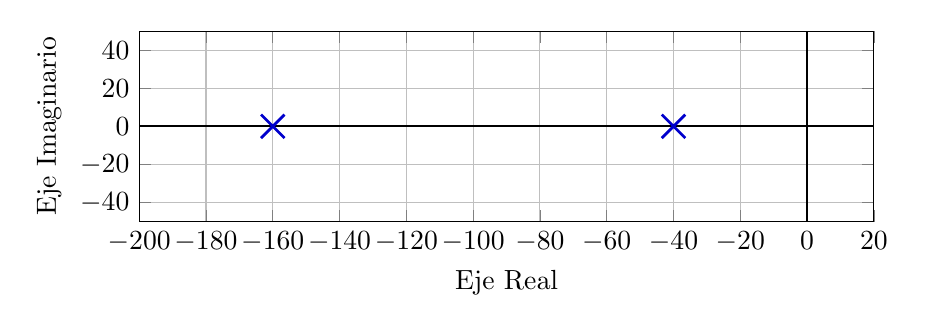
\begin{tikzpicture}
  \begin{axis}[
    width=0.9\columnwidth,
    height=4cm,
    xlabel={Eje Real},
    ylabel={Eje Imaginario},
    grid=both,
    xmin=-200, xmax=20,
    ymin=-50, ymax=50,
  ]
  % Thick x-axis (y=0)
\addplot[
    black,
    line width=0.8pt,
    forget plot
] coordinates {
    (-200,0)
    (20,0)
};

% Thick y-axis (x=0)
\addplot[
    black,
    line width=0.7pt,
    forget plot
] coordinates {
    (0,-50)
    (0,50)
};

    \addplot[
      scatter,
      only marks,
      mark=x,
      mark size=6pt,
      line width=1pt,
      blue,
    ]coordinates{
      (-160,0)
      (-40,0)
    };
  \end{axis}
\end{tikzpicture}

  \caption{Polos en el plano complejo de la FDT.}
  \label{plot:poles_circuito_3}
\end{figure}

Se procede ahora a analizar la FDT en el dominio de la frecuencia reemplazando $s = j\omega$:
\begin{align}
  H(j\omega) &= -\frac{3200 \cdot j\omega}{(j\omega)^2 + 200 \cdot j\omega + 6400} \\
             &= \frac{-3200 \cdot j\omega}{-\omega^2 + 200 \cdot j\omega + 6400}
  \label{eq:fdt-dominio-freq-circuito-3}
\end{align}

Para evaluar los límites de la función de transferencia:
\begin{equation}
  \lim_{\omega \to 0} H(j\omega) = 0
  \qquad \text{y} \qquad
  \lim_{\omega \to \infty} H(j\omega) = 0
\end{equation}
Este comportamiento es el esperado para un filtro pasa banda.

Para el diagrama polar, se separa $H(j\omega)$ en sus componentes real e imaginaria multiplicando y dividiendo por el conjugado del denominador:
\begin{align}
  Re(\omega) &= - \frac{640000 \cdot \omega^2}{\omega^4 + 27200 \cdot \omega^2 + 40960000}\\
  Img(\omega) &= - \frac{3200 \cdot \omega \cdot (6400 - \omega^2)}{\omega^4 + 27200 \cdot \omega^2 + 40960000}
\end{align}

% TODO: El usuario insertará la imagen sacada de LTSpice para el diagrama polar. Se deja el espacio comentado.
\begin{figure}[H]
  \centering
  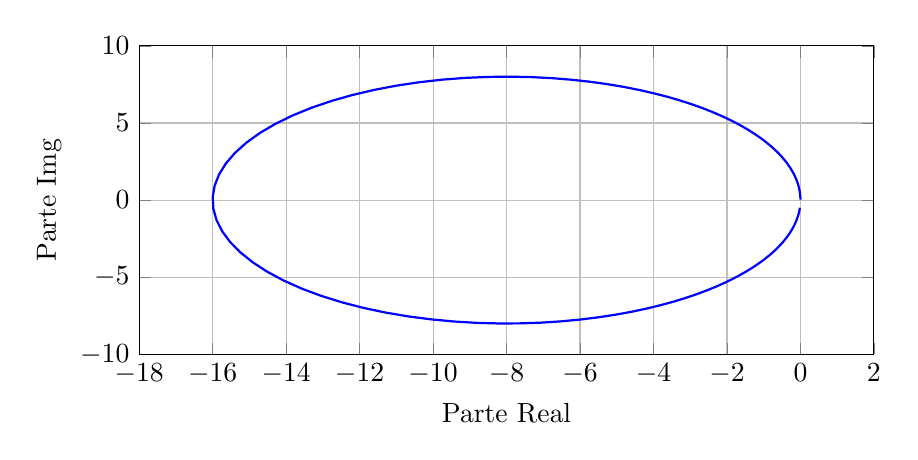
\begin{tikzpicture}
  \begin{axis}[
    width=0.9\columnwidth,
    height=5.5cm,
    xlabel={Parte Real},
    ylabel={Parte Img},
    grid=both,
    xmin=-18, xmax=2,
    ymin=-10, ymax=10,
  ]
  
  \addplot [
    domain=0:5,
    samples=200,
    variable=\t,
    color=blue,
    thick,
  ] (
    { - (640000 * (10^\t)^2) / ((10^\t)^4 + 27200 * (10^\t)^2 + 40960000) },
    { - (3200 * (10^\t) * (6400 - (10^\t)^2)) / ((10^\t)^4 + 27200 * (10^\t)^2 + 40960000) }
  );

  \end{axis}
\end{tikzpicture}

  % \includegraphics[width=0.9\columnwidth]{images/polar_3.png}
  \caption{Diagrama polar de la FDT (Ideal).}
  \label{plot:polar_circuito_3_ideal}
\end{figure}

\begin{figure}[H]
  \centering
  \begin{tikzpicture}
\begin{semilogxaxis}[
    title={Diagrama de Bode de Magnitud},
    xlabel={Frecuencia $\omega$ (rad/s)},
    ylabel={Magnitud (dB)},
    grid=both,
    grid style={line width=.1pt, draw=gray!30},
    major grid style={line width=.2pt, draw=gray!60},
    xmin=1e0, xmax=1e5,
    ymin=-40, ymax=40,
    width=0.9\columnwidth,
    height=8cm,
    legend style={
    nodes={scale=0.7, transform shape}
}
]

\addplot[thick, blue] coordinates {
    (1, -6.02)
    (40, 26.02)
    (160, 26.02)
    (1e5, -29.90)
};
\addlegendentry{Teórico (Asintótico)}

\addplot[mark=*, mark size=1.5pt, red, forget plot] coordinates {(40, 26.02)};
\node[anchor=south east, font=\small, text=black] at (axis cs:40, 26.02) {$\omega_{p1} = 40$};

\addplot[mark=*, mark size=1.5pt, red, forget plot] coordinates {(160, 26.02)};
\node[anchor=south west, font=\small, text=black] at (axis cs:160, 26.02) {$\omega_{p2} = 160$};

% Datos de LTSpice
\addplot[thick, dashed, orange] table [
    skip first n=1,
    x expr=\thisrowno{0} * 2 * pi,
    y index=1
] {sources/circuito3_cleaned.txt};
\addlegendentry{Simulación LTSpice}

\end{semilogxaxis}
\end{tikzpicture}

  \caption{Diagrama de Bode de Magnitud (Real vs Asintótico Ideal).}
  \label{plot:bode_mag_circuito_3}
\end{figure}

\begin{figure}[H]
  \centering
  \begin{tikzpicture}
\begin{semilogxaxis}[
    xlabel={Frecuencia $\omega$ (rad/s)},
    ylabel={Fase (grados)},
    grid=both,
    grid style={line width=.1pt, draw=gray!30},
    major grid style={line width=.2pt, draw=gray!60},
    xmin=1e0, xmax=1e5,
    ymin=-300, ymax=0,
    ytick={0, -90, -180, -270},
    width=0.9\columnwidth,
    height=4.2cm,
    legend style={
    nodes={scale=0.7, transform shape}
}
]

\addplot[thick, blue] coordinates {
    (1, -90)
    (4, -90)
    (16, -117.09)
    (400, -242.90)
    (1600, -270)
    (1e5, -270)
};
\addlegendentry{Teórico (Asintótico)}

\addplot[mark=|, mark size=3pt, red, forget plot] coordinates {(4, -90)};
\node[anchor=south west, font=\small, text=black] at (axis cs:4, -90) {$0.1\omega_{p1}$};

\addplot[mark=|, mark size=3pt, red, forget plot] coordinates {(16, -117.09)};
\node[anchor=south west, font=\small, text=black] at (axis cs:16, -117.09) {$0.1\omega_{p2}$};

% Datos de LTSpice
\addplot[thick, dashed, orange] table [
    skip first n=1,
    x expr=\thisrowno{0} * 2 * pi,
    y index=2
] {sources/circuito3_cleaned.txt};
\addlegendentry{Simulación LTSpice}

\end{semilogxaxis}
\end{tikzpicture}

  \caption{Diagrama de Bode de Fase (Real vs Asintótico Ideal).}
  \label{plot:bode_phase_circuito_3}
\end{figure}


\subsection{Mediciones de Laboratorio}
\label{sec:mediciones_circ_3}

Para la verificación experimental, se realizó la implementación física del filtro pasa banda utilizando componentes reales cuyos valores medidos fueron:
\begin{itemize}
  \item Resistencia $R_1$: $\SI{20}{\kilo\ohm}$ (construida mediante dos resistencias de $\SI{10}{\kilo\ohm}$ en serie)
  \item Resistencia $R_2$: $\SI{400}{\kilo\ohm}$ (construida mediante una resistencia de $\SI{390}{\kilo\ohm}$ y una de $\SI{10}{\kilo\ohm}$ en serie)
  \item Capacitor $C_1$: $\SI{1.2}{\micro\farad}$
  \item Capacitor $C_2$: $\SI{15}{\nano\farad}$
\end{itemize}

El circuito activo fue montado en protoboard utilizando el amplificador operacional JFET dual \textbf{TL082}.

Los capacitores utilizados en el laboratorio ($C_1 = \SI{1.2}{\micro\farad}$ y $C_2 = \SI{15}{\nano\farad}$) son muy cercanos a los valores de diseño teóricos de $\SI{1.25}{\micro\farad}$ y $\SI{15.625}{\nano\farad}$, respectivamente. Con estos componentes reales, la frecuencia angular central teórica $\omega_0$ y la correspondiente frecuencia central de sintonía $f_0$ son:
\begin{align}
  \omega_0 &= \frac{1}{\sqrt{R_1 \cdot C_1 \cdot R_2 \cdot C_2}} \\
           &= \frac{1}{\sqrt{\SI{20}{\kilo\ohm} \cdot \SI{1.2}{\micro\farad} \cdot \SI{400}{\kilo\ohm} \cdot \SI{15}{\nano\farad}}} \approx \SI{83.33}{\radian\per\second}
\end{align}
\begin{equation}
  f_0 = \frac{\omega_0}{2\pi} \approx \SI{13.26}{\hertz}
\end{equation}

Los polos del sistema real se ubican teóricamente en:
\begin{align}
  p_1 &= -\frac{1}{R_1 \cdot C_1} = -\SI{41.67}{\radian\per\second} \quad (f_{p1} \approx \SI{6.63}{\hertz}) \\
  p_2 &= -\frac{1}{R_2 \cdot C_2} = -\SI{166.67}{\radian\per\second} \quad (f_{p2} \approx \SI{26.53}{\hertz})
\end{align}

Durante el ensayo en el laboratorio, se utilizó un generador de señales para aplicar una tensión senoidal $V_{in}$ a la entrada del filtro. Se midieron las tensiones de entrada y salida con un osciloscopio digital RIGOL. Las mediciones originales se registraron en valor pico a pico ($V_{pp}$), con $V_{in} = \SI{2.64}{\volt}_{pp}$ constante para todas las frecuencias. Para la Tabla \ref{tab:mediciones_circuito_3}, los valores fueron convertidos a valor eficaz mediante $V_{rms} = V_{pp}/(2\sqrt{2})$. La ganancia del filtro se expresa directamente en decibeles.

\begin{table}[H]
  \centering
  \begin{tabular}{cccc}
    \hline
    \textbf{Frecuencia} & \textbf{Tensión $V_{in}$ ($V_{rms}$)} & \textbf{Tensión $V_{out}$ ($V_{rms}$)} & \textbf{Ganancia [dB]} \\ \hline
    \SI{1}{\hertz}       & \SI{0.93}{\volt}                      & \SI{1.70}{\volt}                       & \SI{5.19}{\decibel}    \\
    \SI{2}{\hertz}       & \SI{0.93}{\volt}                      & \SI{1.87}{\volt}                       & \SI{6.02}{\decibel}    \\
    \SI{5}{\hertz}       & \SI{0.93}{\volt}                      & \SI{1.92}{\volt}                       & \SI{6.28}{\decibel}    \\
    \SI{8}{\hertz}       & \SI{0.93}{\volt}                      & \SI{1.92}{\volt}                       & \SI{6.28}{\decibel}    \\
    \SI{10}{\hertz}      & \SI{0.93}{\volt}                      & \SI{1.87}{\volt}                       & \SI{6.02}{\decibel}    \\
    \SI{15}{\hertz}      & \SI{0.93}{\volt}                      & \SI{1.75}{\volt}                       & \SI{5.48}{\decibel}    \\
    \SI{20}{\hertz}      & \SI{0.93}{\volt}                      & \SI{1.64}{\volt}                       & \SI{4.90}{\decibel}    \\
    \SI{25}{\hertz}      & \SI{0.93}{\volt}                      & \SI{1.50}{\volt}                       & \SI{4.11}{\decibel}    \\
    \SI{30}{\hertz}      & \SI{0.93}{\volt}                      & \SI{1.41}{\volt}                       & \SI{3.61}{\decibel}    \\
    \SI{45}{\hertz}      & \SI{0.93}{\volt}                      & \SI{1.13}{\volt}                       & \SI{1.67}{\decibel}    \\
    \SI{60}{\hertz}      & \SI{0.93}{\volt}                      & \SI{0.93}{\volt}                       & \SI{0.00}{\decibel}    \\
    \SI{70}{\hertz}      & \SI{0.93}{\volt}                      & \SI{0.79}{\volt}                       & \SI{-1.43}{\decibel}   \\
    \SI{90}{\hertz}      & \SI{0.93}{\volt}                      & \SI{0.68}{\volt}                       & \SI{-2.77}{\decibel}   \\
    \SI{120}{\hertz}     & \SI{0.93}{\volt}                      & \SI{0.57}{\volt}                       & \SI{-4.35}{\decibel}   \\
    \SI{200}{\hertz}     & \SI{0.93}{\volt}                      & \SI{0.35}{\volt}                       & \SI{-8.43}{\decibel}   \\
    \SI{500}{\hertz}     & \SI{0.93}{\volt}                      & \SI{0.14}{\volt}                       & \SI{-16.39}{\decibel}  \\
    \SI{1}{\kilo\hertz}  & \SI{0.93}{\volt}                      & \SI{0.11}{\volt}                       & \SI{-18.89}{\decibel}  \\
    \SI{1}{\mega\hertz}  & \SI{0.93}{\volt}                      & \SI{0.08}{\volt}                       & \SI{-20.83}{\decibel}  \\ \hline
  \end{tabular}
  \caption{Mediciones experimentales del circuito 3 en el laboratorio (convertidas a valor eficaz).}
  \label{tab:mediciones_circuito_3}
\end{table}

\begin{figure}[H]
  \centering
  \begin{tikzpicture}
\begin{semilogxaxis}[
    title={Comparación de Magnitud del Circuito 3 Real},
    xlabel={Frecuencia $\omega$ (rad/s)},
    ylabel={Magnitud (dB)},
    grid=both,
    grid style={line width=.1pt, draw=gray!30},
    major grid style={line width=.2pt, draw=gray!60},
    xmin=1e-1, xmax=1e7,
    ymin=-60, ymax=30,
    width=0.9\columnwidth,
    height=5.5cm,
    legend pos=north east,
    legend style={
        nodes={scale=0.7, transform shape}
    }
]

% Curva de Simulación de LTSpice con Componentes Reales
\addplot[thick, blue] table [
    skip first n=1,
    x expr=\thisrowno{0} * 2 * pi,
    y index=3
] {sources/circuito3_cleaned.txt};
\addlegendentry{Simulación (LTSpice, Real)}

% Puntos Medidos en Laboratorio
\addplot[
    only marks,
    mark=*,
    mark size=2.0pt,
    red
] coordinates {
    (6.283, 5.19)          % 1 Hz
    (12.566, 6.02)         % 2 Hz
    (31.416, 6.28)         % 5 Hz
    (50.265, 6.28)         % 8 Hz
    (62.832, 6.02)         % 10 Hz
    (94.248, 5.48)         % 15 Hz
    (125.664, 4.90)        % 20 Hz
    (157.080, 4.11)        % 25 Hz
    (188.496, 3.61)        % 30 Hz
    (282.743, 1.67)        % 45 Hz
    (376.991, 0.00)        % 60 Hz
    (439.823, -1.43)       % 70 Hz
    (565.487, -2.77)       % 90 Hz
    (753.982, -4.35)       % 120 Hz
    (1256.637, -8.43)      % 200 Hz
    (3141.593, -16.39)     % 500 Hz
    (6283.185, -18.89)     % 1 kHz
    (6283185.307, -20.83)  % 1 MHz
};
\addlegendentry{Mediciones de Laboratorio}

\end{semilogxaxis}
\end{tikzpicture}

  \caption{Comparación entre la simulación de LTSpice del circuito real y las mediciones obtenidas en el laboratorio.}
  \label{plot:bode_medido_vs_teorico_circuito_3}
\end{figure}

A partir de las mediciones graficadas en la Figura \ref{plot:bode_medido_vs_teorico_circuito_3}, se observa el comportamiento característico de un filtro pasa banda. La ganancia máxima medida es de \SI{6.28}{\decibel}, alcanzada entre \SI{5}{\hertz} y \SI{8}{\hertz}, lo que ubica la frecuencia central experimental del filtro en dicho rango. A frecuencias superiores, la atenuación crece progresivamente con una pendiente cercana a \SI{-20}{\decibel} por década, registrándose \SI{-18.89}{\decibel} a \SI{1}{\kilo\hertz} y \SI{-20.83}{\decibel} a \SI{1}{\mega\hertz}.

Para registrar con mayor resolución la respuesta en frecuencia completa del filtro, se capturó la pantalla del osciloscopio mostrada en la Figura \ref{img:fft_circuito_3}, la cual grafica la respuesta obtenida mediante la Transformada Rápida de Fourier (FFT).

\begin{figure}[H]
  \centering
  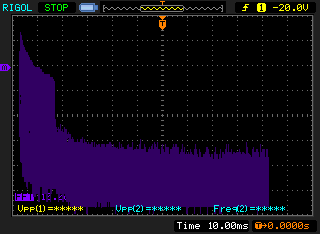
\includegraphics[width=0.9\columnwidth]{images/b3.png}
  \caption{FFT y barrido de frecuencia medido en el laboratorio.}
  \label{img:fft_circuito_3}
\end{figure}

